

\tikzset{every picture/.style={line width=0.75pt}} %set default line width to 0.75pt

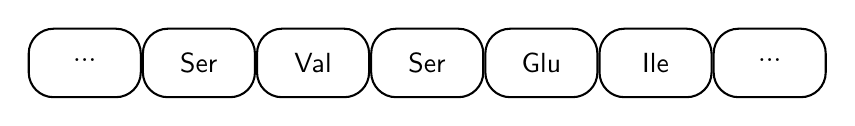
\begin{tikzpicture}[x=0.75pt,y=0.75pt,yscale=-1,xscale=1]
%uncomment if require: \path (0,83); %set diagram left start at 0, and has height of 83


% Text Node
\draw    (78,31) .. controls (78,24.37) and (83.37,19) .. (90,19) -- (120,19) .. controls (126.63,19) and (132,24.37) .. (132,31) -- (132,40) .. controls (132,46.63) and (126.63,52) .. (120,52) -- (90,52) .. controls (83.37,52) and (78,46.63) .. (78,40) -- cycle  ;
\draw (105,35.5) node   [align=left] {\begin{minipage}[lt]{34pt}\setlength\topsep{0pt}
\begin{center}
$\displaystyle \mathsf{Ser}$
\end{center}

\end{minipage}};
% Text Node
\draw    (133,31) .. controls (133,24.37) and (138.37,19) .. (145,19) -- (175,19) .. controls (181.63,19) and (187,24.37) .. (187,31) -- (187,40) .. controls (187,46.63) and (181.63,52) .. (175,52) -- (145,52) .. controls (138.37,52) and (133,46.63) .. (133,40) -- cycle  ;
\draw (160,35.5) node   [align=left] {\begin{minipage}[lt]{34pt}\setlength\topsep{0pt}
\begin{center}
$\displaystyle \mathsf{Val}$
\end{center}

\end{minipage}};
% Text Node
\draw    (188,31) .. controls (188,24.37) and (193.37,19) .. (200,19) -- (230,19) .. controls (236.63,19) and (242,24.37) .. (242,31) -- (242,40) .. controls (242,46.63) and (236.63,52) .. (230,52) -- (200,52) .. controls (193.37,52) and (188,46.63) .. (188,40) -- cycle  ;
\draw (215,35.5) node   [align=left] {\begin{minipage}[lt]{34pt}\setlength\topsep{0pt}
\begin{center}
$\displaystyle \mathsf{Ser}$
\end{center}

\end{minipage}};
% Text Node
\draw    (243,31) .. controls (243,24.37) and (248.37,19) .. (255,19) -- (285,19) .. controls (291.63,19) and (297,24.37) .. (297,31) -- (297,40) .. controls (297,46.63) and (291.63,52) .. (285,52) -- (255,52) .. controls (248.37,52) and (243,46.63) .. (243,40) -- cycle  ;
\draw (270,35.5) node   [align=left] {\begin{minipage}[lt]{34pt}\setlength\topsep{0pt}
\begin{center}
$\displaystyle \mathsf{Glu}$
\end{center}

\end{minipage}};
% Text Node
\draw    (298,31) .. controls (298,24.37) and (303.37,19) .. (310,19) -- (340,19) .. controls (346.63,19) and (352,24.37) .. (352,31) -- (352,40) .. controls (352,46.63) and (346.63,52) .. (340,52) -- (310,52) .. controls (303.37,52) and (298,46.63) .. (298,40) -- cycle  ;
\draw (325,35.5) node   [align=left] {\begin{minipage}[lt]{34pt}\setlength\topsep{0pt}
\begin{center}
$\displaystyle \mathsf{Ile}$
\end{center}

\end{minipage}};
% Text Node
\draw    (23,31) .. controls (23,24.37) and (28.37,19) .. (35,19) -- (65,19) .. controls (71.63,19) and (77,24.37) .. (77,31) -- (77,40) .. controls (77,46.63) and (71.63,52) .. (65,52) -- (35,52) .. controls (28.37,52) and (23,46.63) .. (23,40) -- cycle  ;
\draw (50,35.5) node   [align=left] {\begin{minipage}[lt]{34pt}\setlength\topsep{0pt}
\begin{center}
...
\end{center}

\end{minipage}};
% Text Node
\draw    (353,31) .. controls (353,24.37) and (358.37,19) .. (365,19) -- (395,19) .. controls (401.63,19) and (407,24.37) .. (407,31) -- (407,40) .. controls (407,46.63) and (401.63,52) .. (395,52) -- (365,52) .. controls (358.37,52) and (353,46.63) .. (353,40) -- cycle  ;
\draw (380,35.5) node   [align=left] {\begin{minipage}[lt]{34pt}\setlength\topsep{0pt}
\begin{center}
...
\end{center}

\end{minipage}};


\end{tikzpicture}